\documentclass[10pt,journal,twoside]{IEEEtran}
\usepackage[T1]{fontenc}
\usepackage[utf8]{inputenc}
\usepackage{newtxtext,newtxmath}
\usepackage{graphicx,booktabs,tabularx,array,amsmath,tikz}
\usepackage[hyphens]{url}
\usepackage[hidelinks,breaklinks,hypertexnames=false]{hyperref}
\usepackage{placeins,float}
\usepackage{listings}
\lstset{basicstyle=\ttfamily\scriptsize,breaklines=true,columns=fullflexible,keepspaces=true,frame=single}
\setlength{\emergencystretch}{2em}
\hyphenation{Tensor-Flow Py-Torch scikit-learn}
\pagestyle{plain}
\begin{document}
\raggedbottom


\title{Re-evaluating neural networks for solar power estimation: features, baselines and held-out-day validation}

\author{Oluwafisayo Ibrahim}

\maketitle

\begin{abstract}Neural networks offered no consistent advantage over linear regression in this re-evaluation of solar power estimation. Lower errors with measured current and voltage reflected richer input information rather than better weather-only prediction. Using 180 observations across 20 daily files, the study compares two tracks: electrical and environmental inputs (Track A), and environmental inputs with observation hour (Track B). Linear regression, a no-fitting voltage/current product baseline for Track A, and scikit-learn, TensorFlow/Keras and PyTorch networks are evaluated using seven outer grouped folds, nested selection where applicable, and three neural-network seeds. Metrics pool held-out predictions for each seed. The electrical-product baseline has mean MAE 1.115 W. Track A linear regression achieves mean MAE 0.978 W, compared with 1.334 W for TensorFlow and 1.624 W for PyTorch. In Track B, linear regression achieves mean MAE 11.835 W, compared with 12.179 W for the tuned scikit-learn network. These differences are descriptive. One repeated daily file was excluded before evaluation. Small sample size, uncertain temporal coverage and absent external validation restrict generalisation. Both tracks estimate power from contemporaneous measurements; neither establishes future forecasting capability.\end{abstract}

\begin{IEEEkeywords}Photovoltaic power; neural networks; feature availability; grouped cross-validation; baselines; reproducibility\end{IEEEkeywords}

\section{Introduction}


Photovoltaic power forecasting supports the scheduling and integration of variable solar generation.
Forecasting studies must specify both the prediction horizon and the information available before
that horizon; weather measurements, weather forecasts and electrical measurements imply different
prediction problems \cite{ref2}.

The original undergraduate investigation at Olabisi Onabanjo University used a MATLAB
feedforward ANN to estimate power from measured conditions \cite{ref1}.
The subsequent Python study revisited its task definition, evaluation and baseline comparisons.
It asks whether low errors reflect useful generalisation or access to electrical measurements
that already constrain the target. It also examines whether network complexity provides value
relative to linear regression under the same source-day splits.

\textbf{Research questions.} RQ1: What changes when measured electrical inputs are included?
RQ2: How do ANNs compare with linear and electrical physics baselines within each track?
RQ3: What performance is obtained on held-out source-day groups?
RQ4: How consistent are matched TensorFlow/Keras and PyTorch results across the recorded seeds?
These are questions about this dataset and protocol, rather than claims of a new forecasting algorithm.


\begin{figure}[!t]\centering

\resizebox{\columnwidth}{!}{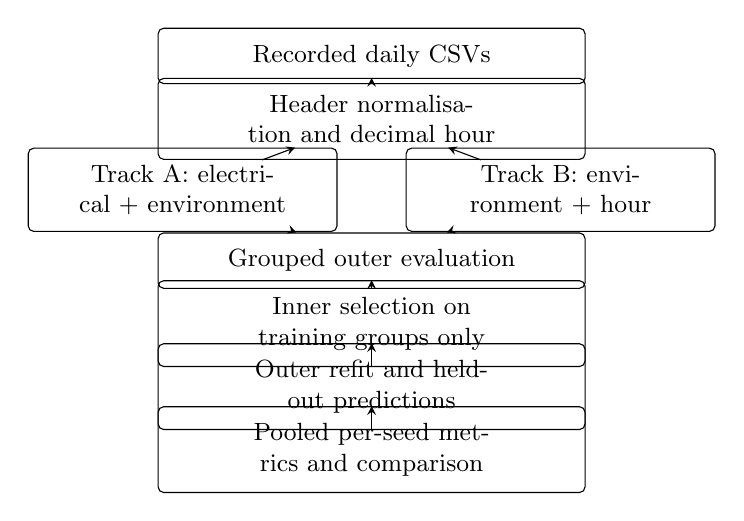
\begin{tikzpicture}[every node/.style={draw,rounded corners=2pt,align=center,font=\small,inner sep=6pt},>=stealth]
\node[text width=5.0cm] (raw) at (0,0) {Recorded daily CSVs};
\node[text width=5.0cm] (prep) at (0,-0.8) {Header normalisation and decimal hour};
\node[text width=3.5cm] (a) at (-2.4,-1.7) {Track A: electrical + environment};
\node[text width=3.5cm] (b) at (2.4,-1.7) {Track B: environment + hour};
\node[text width=5.0cm] (outer) at (0,-2.6) {Grouped outer evaluation};
\node[text width=5.0cm] (inner) at (0,-3.4) {Inner selection on training groups only};
\node[text width=5.0cm] (refit) at (0,-4.2) {Outer refit and held-out predictions};
\node[text width=5.0cm] (score) at (0,-5) {Pooled per-seed metrics and comparison};
\draw[->] (raw) -- (prep);
\draw[->] (prep) -- (a);
\draw[->] (prep) -- (b);
\draw[->] (a) -- (outer);
\draw[->] (b) -- (outer);
\draw[->] (outer) -- (inner);
\draw[->] (inner) -- (refit);
\draw[->] (refit) -- (score);
\end{tikzpicture}}

\caption{Experimental workflow of the Python re-evaluation. Arrows indicate processing stages, not a time-horizon forecast. The two feature configurations enter the same evaluation structure. Model selection is confined to the outer training groups; the final comparison uses saved held-out predictions.\newline\textit{Source:} src/\allowbreak{}load\_data.py; src/\allowbreak{}features.py; src/\allowbreak{}train\_ann\_tf.py; src/\allowbreak{}train\_ann\_torch.py.}

\label{fig:1}

\end{figure}

\section{Related work}


\textbf{Solar prediction and feature availability.} Antonanzas et al. classify photovoltaic forecasting
studies by forecast horizon and origin of inputs, and propose guidelines for comparability \cite{ref2}.
In the present study, inputs measured at the target time define contemporaneous estimation; neither
track specifies an advance prediction horizon. The distinction between estimation and forecasting therefore depends on when the inputs are available.
The electrical baseline implemented here is the direct product of measured voltage and current;
it is not a weather-driven photovoltaic performance model.

\textbf{Feedforward regression.} Hornik et al. establish approximation properties for sufficiently
large feedforward networks under stated assumptions \cite{ref3}. Representational capacity
does not establish that a particular fitted ANN will generalise from a small solar dataset.
This study therefore evaluates small networks against a simpler linear model instead of treating
nonlinearity as evidence of superior performance.

\textbf{Leakage and structured validation.} Kaufman et al. relate leakage to the modelling goal and
information that is legitimately available \cite{ref4}. Current and voltage are legitimate
inputs for electrical estimation, but unavailable shortcuts for a weather-only deployment.
This feature-availability issue differs from fitting preprocessing on test observations.
Roberts et al. explain why validation must respect dependence structures \cite{ref5}.
Here, daily grouping separates measurement days after one repeated daily file was excluded.

\textbf{Selection bias and baseline comparisons.} Cawley and Talbot show that finite-sample model
selection can itself overfit and bias evaluation \cite{ref6}. The Python experiments separate
inner selection from outer scoring and retain simple baselines, shared metrics, configurations
and per-seed predictions. These design choices make the comparisons inspectable; they do not
remove all uncertainty from repeated development on one dataset.


\section{Materials and methods}

\subsection{Dataset, provenance and quality}

The processed dataset contains \textbf{180 observations in 20 daily-file groups}, with nine readings per group. Project documentation attributes the measurements to a solar installation at Olabisi Onabanjo University, Ogun State, Nigeria. The raw daily CSVs accompany the processed dataset, but their exact collection dates cannot be reconstructed from the placeholder timestamps.

Consecutive within-file intervals range from \textbf{35 to 92 minutes}. There are 0 missing cells and 0 exact full-record duplicates when source identity is included. These counts do not establish independence or instrument accuracy.

One repeated daily file was excluded before evaluation. The active dataset contains no exact repeated measurement records when filename identity is excluded. Earlier experiments are retained separately as historical results.

\begin{table*}[!t]
\caption{Observed variables, units and empirical ranges; all stored rows retained.}
\label{tab:1}
\centering\footnotesize
\setlength{\tabcolsep}{4pt}
\renewcommand{\arraystretch}{1.18}
\begin{tabularx}{\textwidth}{>{\hsize=1.696\hsize\linewidth=\hsize\raggedright\arraybackslash}X >{\hsize=0.625\hsize\linewidth=\hsize\raggedright\arraybackslash}X >{\hsize=0.893\hsize\linewidth=\hsize\raggedright\arraybackslash}X >{\hsize=0.893\hsize\linewidth=\hsize\raggedright\arraybackslash}X >{\hsize=0.893\hsize\linewidth=\hsize\raggedright\arraybackslash}X}
\toprule
\textbf{Variable} & \textbf{Unit} & \textbf{Minimum} & \textbf{Median} & \textbf{Maximum} \\ \midrule
Solar irradiance & W/m2 & 254.760 & 894.545 & 1117.750 \\
Temperature & deg C & 24.000 & 32.000 & 36.000 \\
Humidity & \% & 24.000 & 64.000 & 94.000 \\
Current & A & 6.300 & 7.930 & 8.390 \\
Voltage & V & 30.050 & 34.130 & 36.960 \\
Power & W & 189.010 & 270.150 & 300.380 \\
Hour & hour & 8.083 & 12.258 & 16.333 \\
\bottomrule\end{tabularx}
\par\smallskip{\scriptsize Source: data/\allowbreak{}processed/\allowbreak{}solar\_data\_combined.csv. Hour is decimal time; irradiance units follow repository documentation.}
\end{table*}

\begin{figure}[!t]\centering

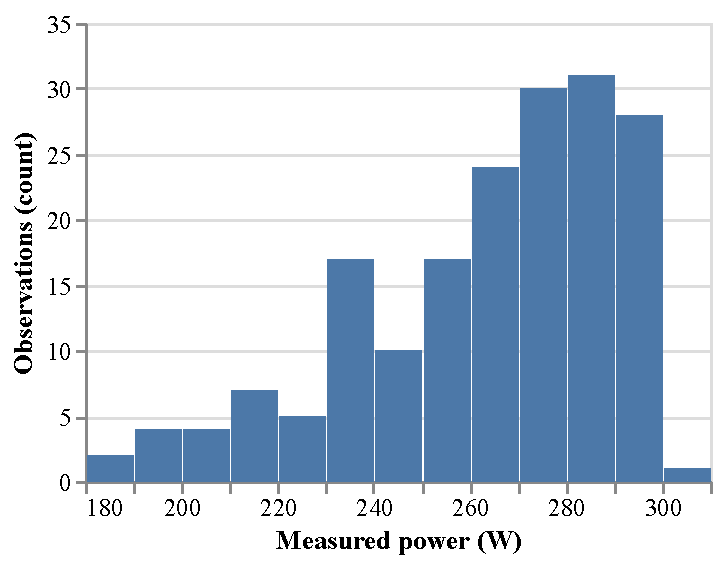
\includegraphics[width=\columnwidth]{figures/figure_2}

\caption{Distribution of measured electrical power across all stored observations, after exclusion of the repeated daily file. Measured power spans 189.01--300.38 W. This is the observed operating range, not evidence of behaviour at night or across other installations.\newline\textit{Source:} data/\allowbreak{}processed/\allowbreak{}solar\_data\_combined.csv; bins summarise counts, not independent days.}

\label{fig:2}

\end{figure}

\subsection{Original MATLAB implementation}


The original model used a ten-neuron feedforward network built with \texttt{fitnet(10)} and trained with Levenberg--Marquardt optimisation. The project description reports \texttt{tansig} hidden activations, a \texttt{purelin} output and daily \texttt{mapminmax} normalisation, together with observation-level random splitting and reuse of daily observations for training and testing.

The available \href{https://github.com/OluwafisayoIbrahim/ANN-Forecasting-for-Solar-Power/blob/578401bb0d106c53f0e152380441a8338854ed57/NeuralNet.m}{NeuralNet.m} script combines five daily files, applies an external 80/10/10 random split and sets a 9,000-epoch training cap. It converts time to numeric form and includes it alongside the five measured predictors. Internal \texttt{fitnet} division is not disabled. The daily training function is not included in the available code, so its reported activations and normalisation cannot be confirmed from that script.

The original preprint \cite{ref1} describes this investigation. Its full text and historical held-out predictions were unavailable, so its numerical results are not used as a comparable benchmark here.

\subsection{Methodological reassessment}

\begin{equation}P=V\times I\end{equation}

{\footnotesize P: electrical power (W); V: voltage (V); I: current (A).\par}


The baseline relation $P=VI$ makes the task definition consequential. Contemporaneous electrical
inputs strongly constrain measured power. That is \textbf{feature--target dependence}, not by itself
proof that test observations contaminated training. It becomes potential target leakage if
those inputs would be unavailable for the stated deployment objective \cite{ref4}.
\textbf{Preprocessing leakage} instead occurs when held-out data influence fitted transformations;
the Python fold-level scalers address that separate issue. \textbf{Observation overlap} is another
problem: identical records under different source identifiers can cross nominal group boundaries.

Track A examines electrical-input estimation. Track B evaluates estimation without current and
voltage, but still uses contemporaneous environmental measurements. The error levels of the two
tracks cannot be interpreted as a fair contest between models with the same information budget.
Neither experiment defines an advance forecasting horizon.


\subsection{Experimental tracks}

Table~\ref{tab:2} defines the two feature sets. Track A includes measured current and voltage alongside environmental variables; Track B excludes electrical measurements and adds observation hour. Both tracks estimate power at the time of measurement, so model comparisons are made within each track.

\begin{table*}[!t]
\caption{Feature sets and legitimate task interpretations.}
\label{tab:2}
\centering\footnotesize
\setlength{\tabcolsep}{4pt}
\renewcommand{\arraystretch}{1.18}
\begin{tabularx}{\textwidth}{>{\hsize=0.643\hsize\linewidth=\hsize\raggedright\arraybackslash}X >{\hsize=1.071\hsize\linewidth=\hsize\raggedright\arraybackslash}X >{\hsize=1.286\hsize\linewidth=\hsize\raggedright\arraybackslash}X}
\toprule
\textbf{Track} & \textbf{Inputs} & \textbf{Interpretation} \\ \midrule
A --- electrical-input replication & solar\_irradiance, current, voltage, temperature, humidity & Power estimation with measured current and voltage \\
B --- environmental/time & solar\_irradiance, temperature, humidity, hour & Power estimation from contemporaneous environmental conditions and time \\
\bottomrule\end{tabularx}
\par\smallskip{\scriptsize Source: src/\allowbreak{}features.py; electrical physics uses only current and voltage in Track A.}
\end{table*}

\subsection{Data preparation and preprocessing}


\texttt{src/load\_data.py} normalises headers, concatenates daily CSVs and adds source filenames.
It parses time using \texttt{\%H:\%M}, constructs decimal hour as hour + minute/60, and adds
calculated power and measured-minus-calculated power diagnostics. The diagnostic columns,
source identifier and placeholder date are excluded from model inputs (\texttt{src/features.py}).
No outlier-removal or imputation procedure is implemented in this preparation path; extreme
values are retained. Missing-value reporting is diagnostic rather than a missing-data model.

The scikit-learn MLP pipeline fits \texttt{StandardScaler} on each training partition; targets remain
in watts. The matched-run linear pipeline also standardises inputs. TensorFlow/PyTorch fit
separate input and target standardisers on training observations only, transform validation
inputs using those fitted values, and inverse-transform outputs to watts. Inner models and
outer refits obtain fresh scalers. The historical \texttt{src/baselines.py} also contains an in-sample
linear check; manuscript scores instead use the saved grouped-CV outputs.


\subsection{Models and baselines}

\begin{table*}[!t]
\caption{Training configurations for the matched S2 comparison; the mean sanity check is not a ranked experiment.}
\label{tab:3}
\centering\footnotesize
\setlength{\tabcolsep}{4pt}
\renewcommand{\arraystretch}{1.18}
\begin{tabularx}{\textwidth}{>{\hsize=0.586\hsize\linewidth=\hsize\raggedright\arraybackslash}X >{\hsize=1.034\hsize\linewidth=\hsize\raggedright\arraybackslash}X >{\hsize=1.379\hsize\linewidth=\hsize\raggedright\arraybackslash}X}
\toprule
\textbf{Model} & \textbf{Architecture / selection} & \textbf{Training} \\ \midrule
Physics (A only) & P = I $\times$ V; no fitted parameters & None \\
Linear (A, B) & Ordinary least squares; no tuning & Training-partition input standardisation \\
scikit-learn untuned (A, B) & 10 tanh units; alpha=0.0001 & L-BFGS, max\_iter=5000; input scaling \\
scikit-learn tuned (A, B) & 3 or 10 tanh units; alpha $\in$ \{0.1, 1, 10\} & 3 inner grouped folds; L-BFGS; input scaling \\
TensorFlow / PyTorch selected (A, B) & [[10], [16, 8]]; tanh; linear output & Adam; lr=0.01; hidden-kernel L2=0.0001; batch=16; cap=1000; patience=30; input/target scaling \\
Mean prediction & Metric sanity check only (src/evaluate.py) & No saved grouped-CV experiment; excluded from result rankings \\
\bottomrule\end{tabularx}
\par\smallskip{\scriptsize Source: src/\allowbreak{}models.py; src/\allowbreak{}models\_tf.py; src/\allowbreak{}models\_torch.py; both S2 config.json files; src/\allowbreak{}evaluate.py.}
\end{table*}

Both neural frameworks use MSE on standardised targets plus hidden-kernel L2, excluding output kernels and biases. The PyTorch implementation explicitly uses Glorot-uniform kernels, zero biases, seeded shuffled batches, Adam epsilon 1e-7, no optimiser weight decay, and deterministic single-thread CPU execution. Keras uses its Dense initialisation and Adam implementation. Shared settings do not imply identical numerical optimisation. The scikit-learn MLP is a practical approximation of the historical network, not an implementation of MATLAB trainlm.

\subsection{Grouped validation and model selection}


Seven outer \texttt{GroupKFold} partitions evaluate 180 observations across 20 daily files. Six folds hold out three groups (27 rows) and train on 17 groups (153 rows); one holds out two groups (18 rows) and trains on 18 groups (162 rows). Each row receives one outer prediction per model and seed. Three inner grouped folds use 11 or 12 fitting groups and six or five validation groups when the outer training set has 17 groups; with 18 groups, they use 12 and six.
The tuned scikit-learn MLP selects hidden size and alpha by mean inner MAE; its untuned
reference has fixed settings. Linear regression has no nested search; the physics product
has no fitted parameters.

TensorFlow/PyTorch select architecture by mean inner MAE in watts. Within each inner fit,
validation MAE controls early stopping; best weights are restored. The median best epoch
of the selected architecture's inner folds determines the outer training-only refit duration.
This reuses inner validation for stopping and selection, which can favour optimistic inner
scores. Outer test rows do not choose the architecture or epochs.

Seeds 0, 1 and 2 vary ANN initialisation. Scores pool all outer predictions per seed before
computing a mean and population standard deviation across seeds. Deterministic baselines
repeat the same values across these records. These are not confidence intervals or
independent dataset replications. Training and test partitions share neither a daily group nor an exact measurement record. This does not establish independence across sites or seasons.

S1 and S2 were compared using a documented cap-hit rule and inner evidence, rather than choosing
the lowest outer error. S2 was selected. Historical outer scores had already been inspected,
so this remains a development study requiring independent confirmation. Matching framework
settings does not make random initialisations or floating-point operations identical.


\textbf{S1/S2 convergence diagnostics.} Across both tracks, S1 had 2 selected outer refits at the epoch cap and S2 had 0. S1 used batch size 32 and S2 used 16; all other training settings matched. The tie-breakers were lower equal-track mean inner MAE, followed by S1 for an exact tie. The selection rule preferred fewer total cap hits, so S2 was selected using inner evidence. The screening threshold is fewer than 20\% of selected refits at the cap per track. Reaching the cap can indicate undertraining; avoiding it or passing this screen does not prove convergence. These counts come from the saved selected settings, not outer-test accuracy.

\begin{figure}[!t]\centering

\resizebox{\columnwidth}{!}{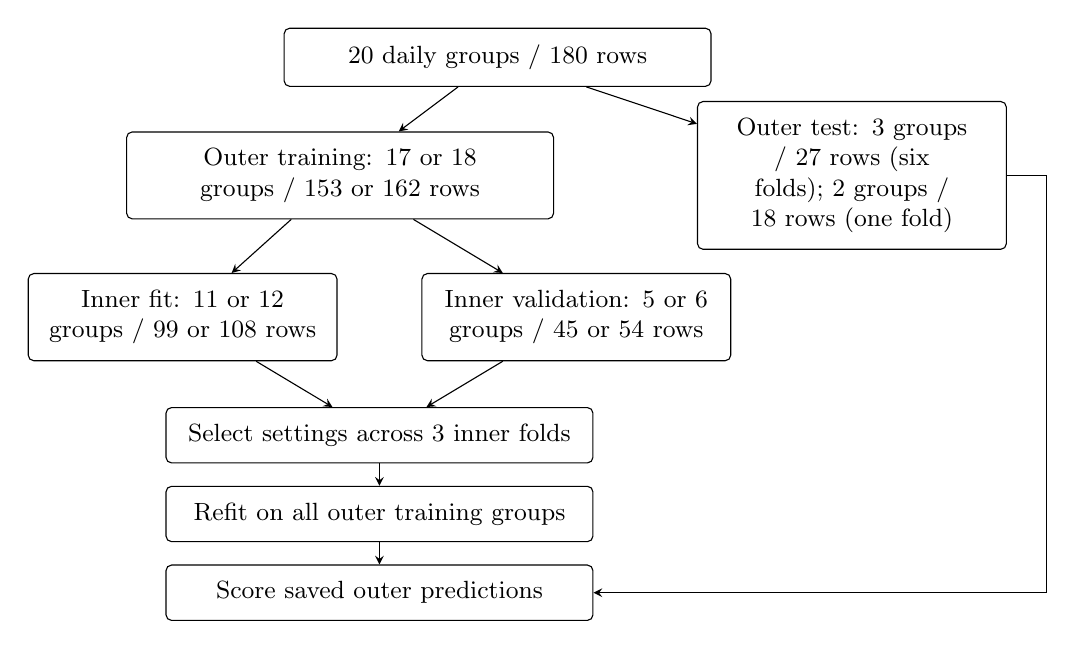
\begin{tikzpicture}[every node/.style={draw,rounded corners=2pt,align=center,font=\small,inner sep=6pt},>=stealth]
\node[text width=5.0cm] (raw) at (0,0) {20 daily groups / 180 rows};
\node[text width=5.0cm] (train) at (-2,-1.5) {Outer training: 17 or 18 groups / 153 or 162 rows};
\node[text width=3.5cm] (test) at (4.5,-1.5) {Outer test: 3 groups / 27 rows (six folds); 2 groups / 18 rows (one fold)};
\node[text width=3.5cm] (fit) at (-4,-3.3) {Inner fit: 11 or 12 groups / 99 or 108 rows};
\node[text width=3.5cm] (val) at (1,-3.3) {Inner validation: 5 or 6 groups / 45 or 54 rows};
\node[text width=5.0cm] (select) at (-1.5,-4.8) {Select settings across 3 inner folds};
\node[text width=5.0cm] (refit) at (-1.5,-5.8) {Refit on all outer training groups};
\node[text width=5.0cm] (score) at (-1.5,-6.8) {Score saved outer predictions};
\draw[->] (raw) -- (train);
\draw[->] (raw) -- (test);
\draw[->] (train) -- (fit);
\draw[->] (train) -- (val);
\draw[->] (fit) -- (select);
\draw[->] (val) -- (select);
\draw[->] (select) -- (refit);
\draw[->] (refit) -- (score);
\draw[->] (test.east) -- ++(.5,0) |- (score.east);
\end{tikzpicture}}

\caption{One outer iteration of the nested grouped design; repeat for seven outer folds and each ANN seed. The outer test branch does not enter inner selection. Counts refer to filename groups, not verified independent dates; test daily groups and identical measurement records are excluded from fitting. Inner branches rotate over three partitions.\newline\textit{Source:} src/\allowbreak{}train\_ann.py; src/\allowbreak{}train\_ann\_tf.py; saved S2 configurations and fold assignments.}

\label{fig:3}

\end{figure}

\subsection{Metrics and aggregation}

Let $y_i$ and $\hat y_i$ be measured and predicted power in watts, $n$ the number of pooled held-out rows, $\bar y$ their measured mean and $S=\{i:y_i\ne0\}$. Each seed pools all outer rows before scoring.

\begin{equation}\mathrm{MAE}=\frac{1}{n}\sum_{i=1}^{n}|y_i-\hat y_i|\end{equation}

{\footnotesize MAE (W): average absolute error.\par}

\begin{equation}\mathrm{RMSE}=\sqrt{\frac{1}{n}\sum_{i=1}^{n}(y_i-\hat y_i)^2}\end{equation}

{\footnotesize RMSE (W): gives larger errors greater influence.\par}

\begin{equation}\mathrm{MAPE}=\frac{100}{|S|}\sum_{i\in S}\left|\frac{y_i-\hat y_i}{y_i}\right|\end{equation}

{\footnotesize MAPE (\%): zero measured values are excluded; small nonzero denominators can dominate. Undefined if S is empty.\par}

\begin{equation}R^2=1-\frac{\sum_i(y_i-\hat y_i)^2}{\sum_i(y_i-\bar y)^2}\end{equation}

{\footnotesize R$^2$ (unitless): may be negative; the manuscript treats constant-target R$^2$ as undefined.\par}

MAE, RMSE and MAPE favour lower values; R$^2$ favours higher values. Tables report mean $\pm$ population seed standard deviation (\texttt{ddof=0}), not the average or spread of fold metrics. The mean-prediction code in \texttt{src/evaluate.py} is a synthetic metric check, not a fitted outer-training-mean baseline experiment.

\section{Experimental results}

Tables IV--VI report the matched S2 experiments. Scores are calculated from saved out-of-fold predictions and summarised across seeds. The active evaluation contains no repeated measurement records across the training/test partitions.

\subsection{Historical findings and comparability}

Historical MATLAB results cannot be compared directly with these experiments because the original full text and held-out prediction records were unavailable. Earlier Python and TensorFlow runs use different training settings and are excluded from the matched S2 comparison.

\subsection{Track A}

\begin{table*}[!t]
\caption{Track A: pooled out-of-fold performance, mean $\pm$ population standard deviation across seeds.}
\label{tab:4}
\centering\footnotesize
\setlength{\tabcolsep}{4pt}
\renewcommand{\arraystretch}{1.18}
\begin{tabularx}{\textwidth}{>{\hsize=1.250\hsize\linewidth=\hsize\raggedright\arraybackslash}X >{\hsize=0.938\hsize\linewidth=\hsize\raggedright\arraybackslash}X >{\hsize=0.938\hsize\linewidth=\hsize\raggedright\arraybackslash}X >{\hsize=0.938\hsize\linewidth=\hsize\raggedright\arraybackslash}X >{\hsize=0.938\hsize\linewidth=\hsize\raggedright\arraybackslash}X}
\toprule
\textbf{Model} & \textbf{MAE (W)} & \textbf{RMSE (W)} & \textbf{MAPE (\%)} & \textbf{R$^2$} \\ \midrule
Linear & 0.978 $\pm$ 0.000 & 1.235 $\pm$ 0.000 & 0.377 $\pm$ 0.000 & 0.998 $\pm$ 0.000 \\
Physics & 1.115 $\pm$ 0.000 & 1.254 $\pm$ 0.000 & 0.424 $\pm$ 0.000 & 0.998 $\pm$ 0.000 \\
PyTorch selected & 1.624 $\pm$ 0.148 & 2.405 $\pm$ 0.145 & 0.622 $\pm$ 0.062 & 0.992 $\pm$ 0.001 \\
Sklearn tuned & 1.069 $\pm$ 0.060 & 1.393 $\pm$ 0.089 & 0.413 $\pm$ 0.026 & 0.997 $\pm$ 0.000 \\
Sklearn untuned & 1.304 $\pm$ 0.538 & 3.580 $\pm$ 3.118 & 0.505 $\pm$ 0.214 & 0.970 $\pm$ 0.039 \\
TensorFlow selected & 1.334 $\pm$ 0.159 & 1.863 $\pm$ 0.297 & 0.515 $\pm$ 0.059 & 0.995 $\pm$ 0.002 \\
\bottomrule\end{tabularx}
\par\smallskip{\scriptsize Source: results/\allowbreak{}research\_20\_days/\allowbreak{}comparison/\allowbreak{}comparison.csv}
\end{table*}

Track A: Linear has the lowest mean MAE (0.978 W); linear regression has mean MAE 0.978 W. Differences are descriptive; no significance test is supplied. The electrical-product baseline already gives low error without learning.

\subsection{Track B}

\begin{table*}[!t]
\caption{Track B: pooled out-of-fold performance, mean $\pm$ population standard deviation across seeds.}
\label{tab:5}
\centering\footnotesize
\setlength{\tabcolsep}{4pt}
\renewcommand{\arraystretch}{1.18}
\begin{tabularx}{\textwidth}{>{\hsize=1.250\hsize\linewidth=\hsize\raggedright\arraybackslash}X >{\hsize=0.938\hsize\linewidth=\hsize\raggedright\arraybackslash}X >{\hsize=0.938\hsize\linewidth=\hsize\raggedright\arraybackslash}X >{\hsize=0.938\hsize\linewidth=\hsize\raggedright\arraybackslash}X >{\hsize=0.938\hsize\linewidth=\hsize\raggedright\arraybackslash}X}
\toprule
\textbf{Model} & \textbf{MAE (W)} & \textbf{RMSE (W)} & \textbf{MAPE (\%)} & \textbf{R$^2$} \\ \midrule
Linear & 11.835 $\pm$ 0.000 & 14.928 $\pm$ 0.000 & 4.724 $\pm$ 0.000 & 0.702 $\pm$ 0.000 \\
PyTorch selected & 12.032 $\pm$ 0.262 & 15.027 $\pm$ 0.246 & 4.806 $\pm$ 0.097 & 0.698 $\pm$ 0.010 \\
Sklearn tuned & 12.179 $\pm$ 0.037 & 15.633 $\pm$ 0.278 & 4.865 $\pm$ 0.012 & 0.673 $\pm$ 0.012 \\
Sklearn untuned & 14.044 $\pm$ 0.267 & 18.890 $\pm$ 1.219 & 5.584 $\pm$ 0.136 & 0.521 $\pm$ 0.063 \\
TensorFlow selected & 11.951 $\pm$ 0.317 & 14.989 $\pm$ 0.372 & 4.761 $\pm$ 0.107 & 0.700 $\pm$ 0.015 \\
\bottomrule\end{tabularx}
\par\smallskip{\scriptsize Source: results/\allowbreak{}research\_20\_days/\allowbreak{}comparison/\allowbreak{}comparison.csv}
\end{table*}

Track B: Linear has the lowest mean MAE (11.835 W); linear regression has mean MAE 11.835 W. Differences are descriptive; no significance test is supplied.

\subsection{Error diagnostics and framework variability}

Figures~\ref{fig:4}--\ref{fig:7} show prediction agreement, mean absolute error across seeds, signed residuals and variation in error between source-file groups. The parity, residual and group-error plots use all held-out predictions from seed 0 for Track B; the comparison plot summarises all three seeds. Table~\ref{tab:6} reports the framework-specific per-seed scores. Together, these diagnostics show differences between individual errors, group-level performance and sensitivity to initialisation.

\begin{figure}[!t]\centering

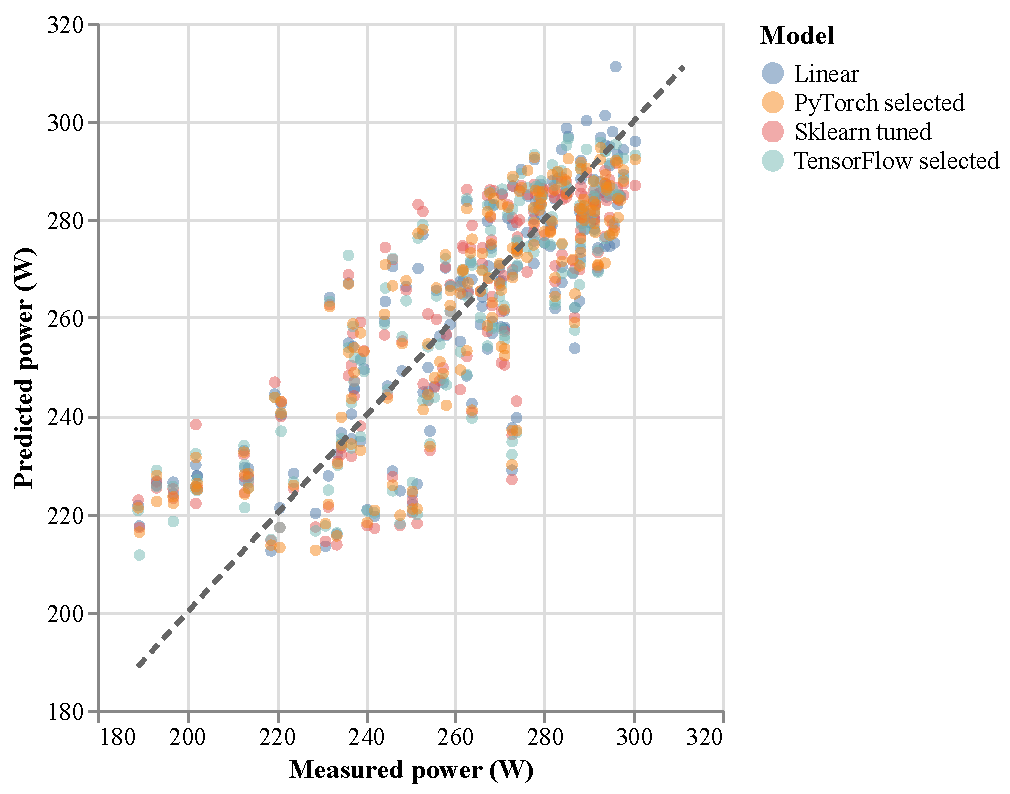
\includegraphics[width=\columnwidth]{figures/figure_4}

\caption{Measured versus predicted power, Track B, seed 0; each model includes every saved outer row. Dashed line: identity. Scatter around the identity line shows individual errors that pooled averages conceal. This disclosed seed is a diagnostic illustration, not a best-seed selection or an independent test of the full-data deployment weights.\newline\textit{Source:} results/\allowbreak{}research\_20\_days/\allowbreak{}tensorflow\_s2/\allowbreak{}predictions.csv; results/\allowbreak{}research\_20\_days/\allowbreak{}pytorch\_selected/\allowbreak{}predictions.csv}

\label{fig:4}

\end{figure}

\begin{figure}[!t]\centering

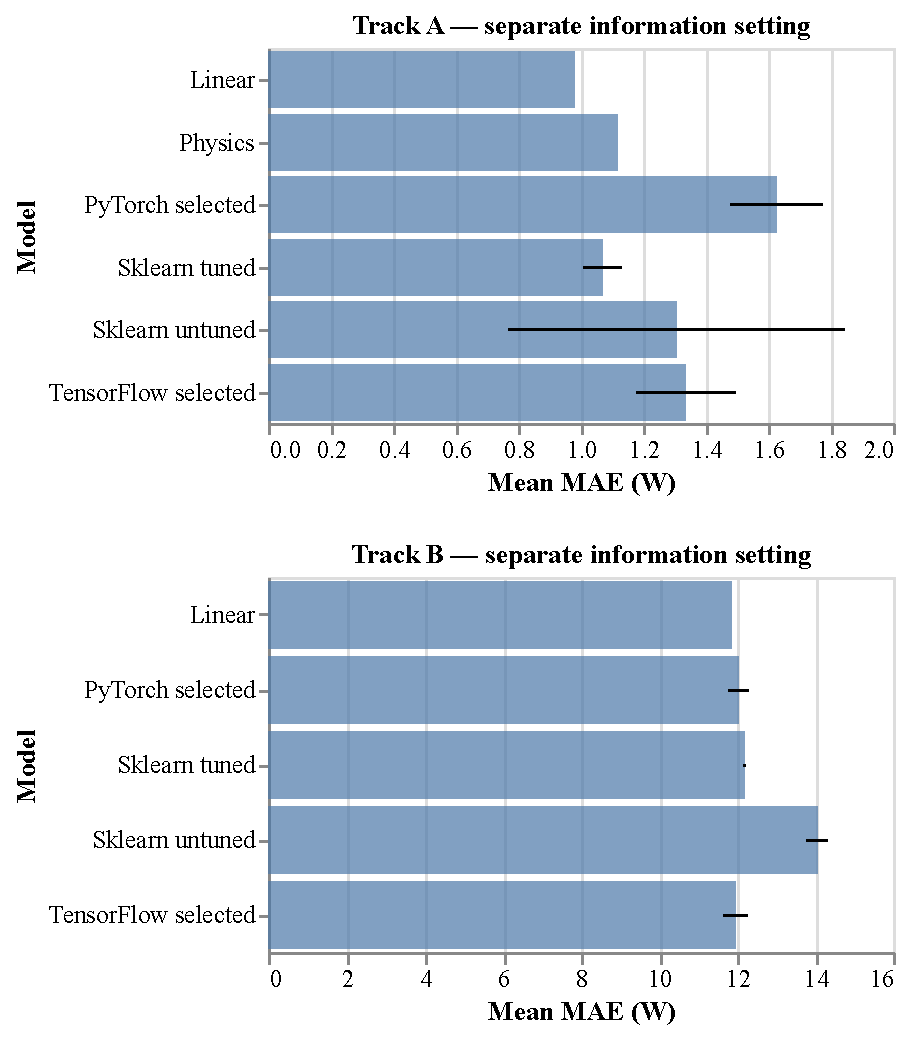
\includegraphics[width=\columnwidth]{figures/figure_5}

\caption{Matched S2 mean MAE with $\pm$ one population seed standard deviation. Track panels use independent scales; bars start at zero. Within-track comparisons hold feature availability fixed. Across-track bar lengths must not be read as a fair contest between equivalent tasks. Whiskers describe three-seed variation, not confidence intervals; near-zero baseline variation reflects repeated deterministic predictions.\newline\textit{Source:} results/\allowbreak{}research\_20\_days/\allowbreak{}comparison/\allowbreak{}comparison.csv}

\label{fig:5}

\end{figure}

\begin{table*}[!t]
\caption{Framework-specific per-seed pooled scores; historical runs excluded.}
\label{tab:6}
\centering\footnotesize
\setlength{\tabcolsep}{4pt}
\renewcommand{\arraystretch}{1.18}
\begin{tabularx}{\textwidth}{>{\hsize=1.055\hsize\linewidth=\hsize\raggedright\arraybackslash}X >{\hsize=0.527\hsize\linewidth=\hsize\raggedright\arraybackslash}X >{\hsize=1.758\hsize\linewidth=\hsize\raggedright\arraybackslash}X >{\hsize=0.440\hsize\linewidth=\hsize\raggedright\arraybackslash}X >{\hsize=1.055\hsize\linewidth=\hsize\raggedright\arraybackslash}X >{\hsize=1.055\hsize\linewidth=\hsize\raggedright\arraybackslash}X >{\hsize=1.055\hsize\linewidth=\hsize\raggedright\arraybackslash}X >{\hsize=1.055\hsize\linewidth=\hsize\raggedright\arraybackslash}X}
\toprule
\textbf{Track} & \textbf{Seed} & \textbf{Model} & \textbf{MAE (W)} & \textbf{RMSE (W)} & \textbf{MAPE (\%)} & \textbf{R$^2$} & \textbf{Framework} \\ \midrule
A & 0 & TensorFlow selected & 1.172 & 1.579 & 0.447 & 0.997 & TensorFlow \\
A & 1 & TensorFlow selected & 1.550 & 2.272 & 0.592 & 0.993 & TensorFlow \\
A & 2 & TensorFlow selected & 1.281 & 1.737 & 0.505 & 0.996 & TensorFlow \\
B & 0 & TensorFlow selected & 12.054 & 15.088 & 4.806 & 0.696 & TensorFlow \\
B & 1 & TensorFlow selected & 11.521 & 14.492 & 4.615 & 0.719 & TensorFlow \\
B & 2 & TensorFlow selected & 12.278 & 15.386 & 4.864 & 0.684 & TensorFlow \\
A & 0 & PyTorch selected & 1.569 & 2.259 & 0.604 & 0.993 & PyTorch \\
A & 1 & PyTorch selected & 1.826 & 2.603 & 0.705 & 0.991 & PyTorch \\
A & 2 & PyTorch selected & 1.477 & 2.353 & 0.557 & 0.993 & PyTorch \\
B & 0 & PyTorch selected & 12.263 & 15.167 & 4.895 & 0.693 & PyTorch \\
B & 1 & PyTorch selected & 12.166 & 15.232 & 4.852 & 0.690 & PyTorch \\
B & 2 & PyTorch selected & 11.665 & 14.681 & 4.672 & 0.712 & PyTorch \\
\bottomrule\end{tabularx}
\par\smallskip{\scriptsize Source: results/\allowbreak{}research\_20\_days/\allowbreak{}tensorflow\_s2/\allowbreak{}metrics\_per\_seed.csv; results/\allowbreak{}research\_20\_days/\allowbreak{}pytorch\_selected/\allowbreak{}metrics\_per\_seed.csv}
\end{table*}

\begin{figure}[!t]\centering

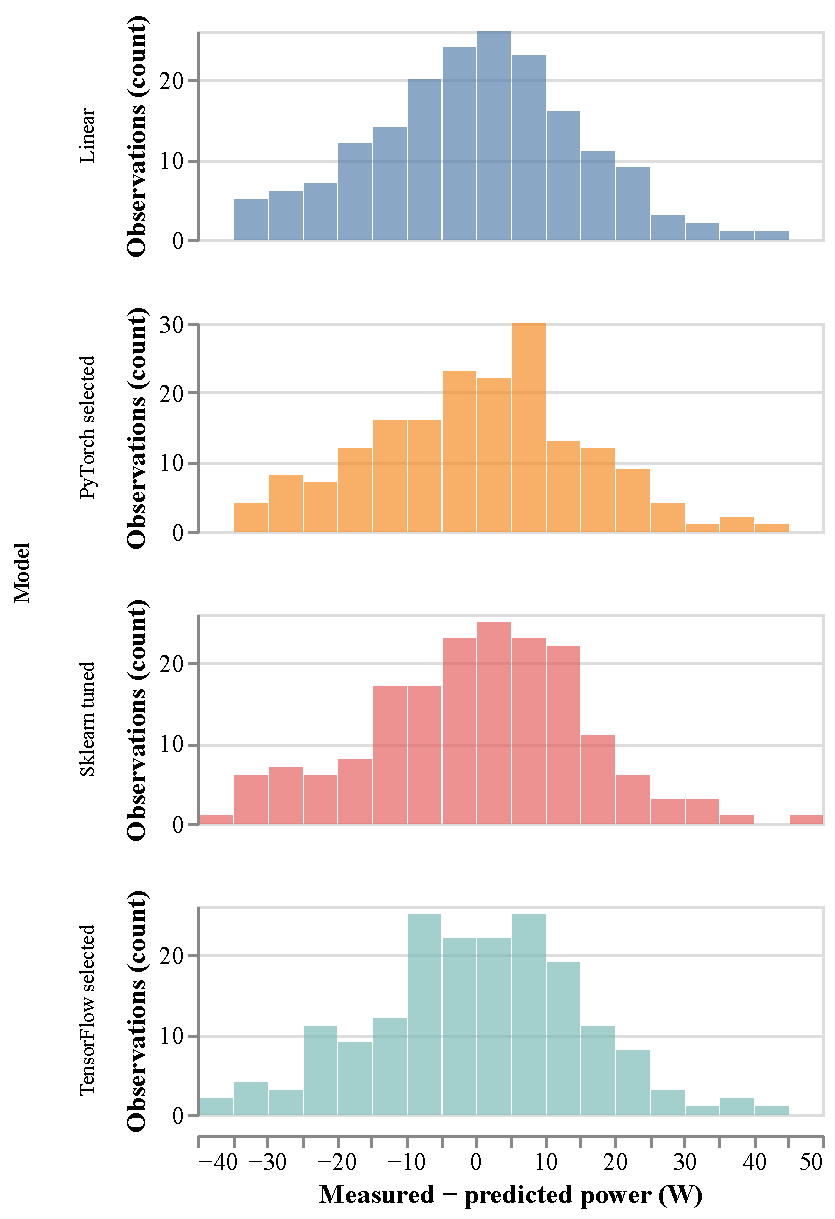
\includegraphics[width=\columnwidth]{figures/figure_6}

\caption{Signed residual histograms, Track B, seed 0. Residual = measured - predicted power; vertical scales vary by model. Negative residuals indicate overestimation; positive residuals indicate underestimation. The distributions expose the balance and spread of errors, but do not provide calibrated uncertainty intervals.\newline\textit{Source:} Saved S2 predictions.csv files; same rows and models as Figure 4.}

\label{fig:6}

\end{figure}

\begin{figure}[!t]\centering

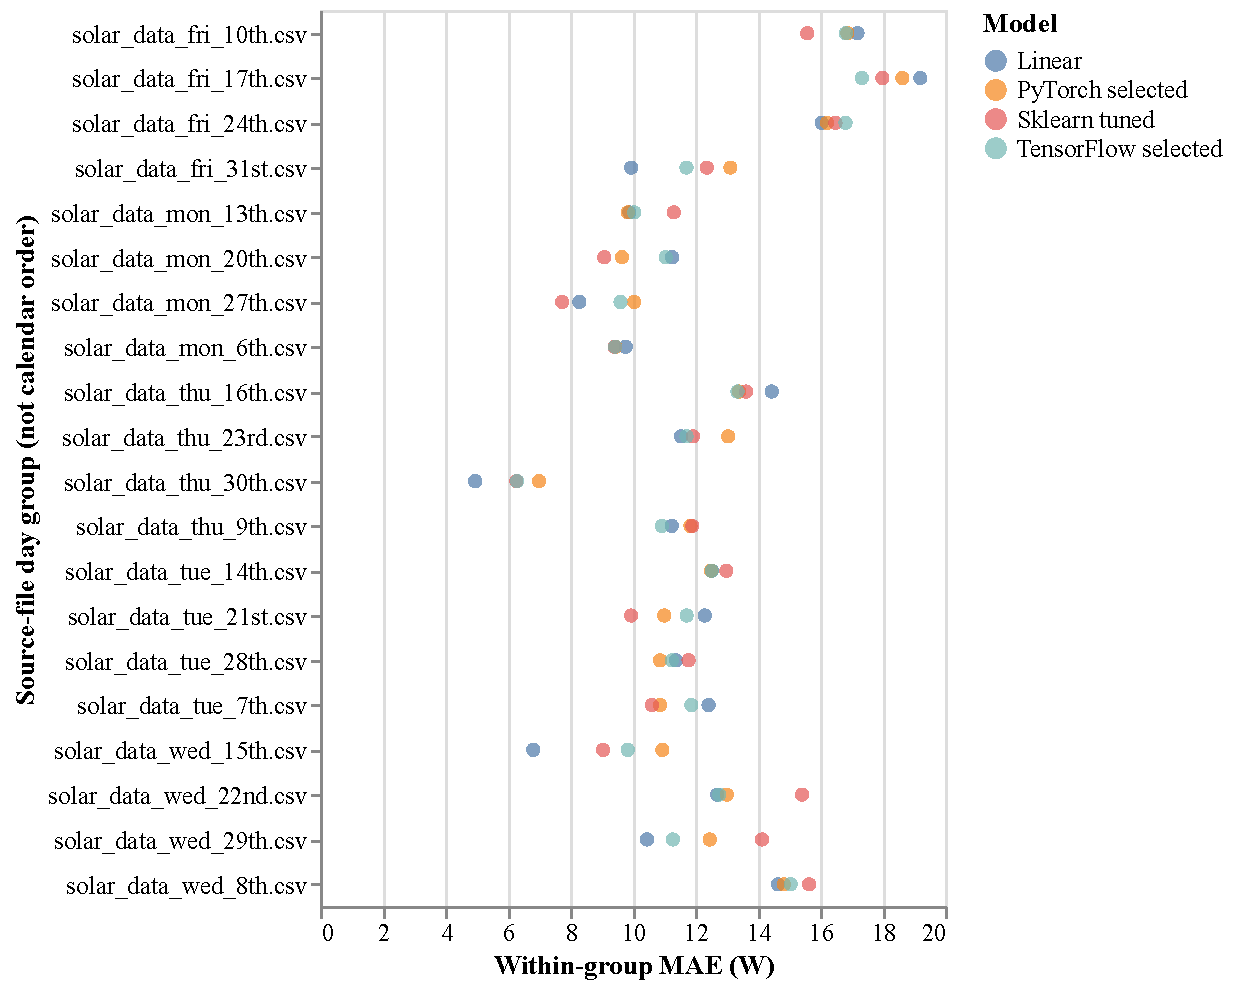
\includegraphics[width=\columnwidth]{figures/figure_7}

\caption{Within-source-group MAE, Track B, seed 0; filename order is categorical rather than chronological. Group-level errors vary across the measurement conditions, which a single pooled score can hide. Each point averages the nine stored readings for one filename and model. These group metrics are descriptive and are not substituted for the pooled per-seed results.\newline\textit{Source:} Saved S2 predictions.csv files; mean absolute residual grouped by day\_id and model.}

\label{fig:7}

\end{figure}

\section{Discussion}

\textbf{RQ1 --- information changes the task.} The mean absolute difference between measured power
and the electrical product is 1.115 W. Track A can exploit this near-identity,
whereas Track B cannot. Lower Track A errors reflect richer contemporaneous information; they are
not evidence of superior weather-only forecasting.

\textbf{RQ2 --- baseline comparisons.} Track A: Linear has the lowest mean MAE (0.978 W); linear regression has mean MAE 0.978 W. Differences are descriptive; no significance test is supplied. Track B: Linear has the lowest mean MAE (11.835 W); linear regression has mean MAE 11.835 W. Differences are descriptive; no significance test is supplied. Rankings depend on the metric and must be interpreted within each track.

\textbf{RQ3 --- held-out days.} Each test daily group and its measurements are excluded from fitting. Model selection is nested within the outer training days. One repeated daily file was excluded before evaluation. There is no controlled experiment isolating the effect of changing the split strategy. External-site or future-horizon performance cannot be inferred from these results.

\textbf{RQ4 --- implementation comparison, not a universal framework ranking.} TensorFlow and PyTorch use
matching recorded settings, reference data and outer assignments. Their error and seed variation
describe this protocol; non-identical initialisations, updates and early stopping can still yield
different fits. The evidence does not establish a statistically supported framework winner or make
software framework choice a substitute for task definition and baseline evaluation.

\section{Limitations}


\textbf{Sample size and effective independence.} Only 180 observations across 20 daily files are available. One repeated daily file was excluded before evaluation. The retained records contain no exact repeated measurements when filename identity is excluded. The small sample and potentially correlated readings still limit generalisation.

\textbf{Temporal and geographic coverage.} Collection is attributed to one university installation
in the project documentation. The processed timestamps contain a placeholder date, and source
names do not establish a full calendar period. Observations are approximately hourly, with
irregular intervals. Cross-season, multi-site and changed-installation performance are untested.

\textbf{Measurement uncertainty.} The original project names measurement instruments, but calibration
records and quantified measurement uncertainty are not available in this repository. Differences
between measured power and $VI$ are observed, but cannot be assigned to a particular instrument
or physical mechanism from these files alone.

\textbf{Deployment information.} Track A requires contemporaneous electrical measurements. Track B
does not, but still requires measured environmental conditions at the target time. Neither has
been validated using advance weather forecasts, independently collected external data, or a
production operational workflow. The interactive app demonstrates inference, not deployment validity.

\textbf{Selection and variability.} Three seeds provide a limited view of initialisation sensitivity.
They do not quantify uncertainty over sites or seasons, and the same small dataset has supported
multiple rounds of development. Historical cap hits and untuned-network instability caution against
equating additional complexity or a completed optimisation run with reliable generalisation.
No confidence intervals, significance tests or calibrated prediction intervals are supplied.


\section{Conclusion and future work}


The principal contribution is a methodological re-evaluation: it separates electrical-input
estimation from environmental/time-based estimation, supplies physics and linear baselines,
and records grouped, nested evaluation across three neural-network implementations. The
saved results do not justify a general claim that ANNs are superior to linear regression,
nor that this system forecasts future solar generation.

\textbf{Proposed work, not completed experiments.} Collect longer records across
seasons and installations, preserve full timestamps and instrument metadata, and evaluate
external datasets. Define one-hour-ahead or day-ahead tasks using only inputs available before
the target time. Compare justified temporal and tree-based baselines; assess uncertainty
calibration and seasonal robustness. Physics-informed learning is a possible extension only
where the available measurements and physical model warrant it.


\section{Research transparency and reproducibility}

\textbf{Data availability.} \href{https://github.com/OluwafisayoIbrahim/solar-power-prediction-python/tree/dev/data/raw}{Raw daily CSVs} and \href{https://github.com/OluwafisayoIbrahim/solar-power-prediction-python/tree/dev/data/processed/solar_data_combined.csv}{processed measurements} are included in the repository. Full calendar dates and instrument calibration records remain unavailable. One repeated daily file was excluded; no missing metadata are inferred from filenames.

\textbf{Code and artifacts.} \href{https://github.com/OluwafisayoIbrahim/solar-power-prediction-python/tree/dev/src}{Python source}, \href{https://github.com/OluwafisayoIbrahim/solar-power-prediction-python/tree/dev/results}{saved experiments} and \href{https://github.com/OluwafisayoIbrahim/solar-power-prediction-python/tree/dev/deployment/}{deployment documentation} are available. Saved model bundles are for inference; their full-data fitted weights do not supply the outer-CV scores in this report.

{\footnotesize Software versions used for the research runs\par}

\begin{table}[H]
\caption{Recorded research-run software versions.}
\label{tab:7}
\centering\footnotesize
\setlength{\tabcolsep}{4pt}
\renewcommand{\arraystretch}{1.18}
\begin{tabularx}{\columnwidth}{>{\hsize=1.000\hsize\linewidth=\hsize\raggedright\arraybackslash}X >{\hsize=1.000\hsize\linewidth=\hsize\raggedright\arraybackslash}X >{\hsize=1.000\hsize\linewidth=\hsize\raggedright\arraybackslash}X >{\hsize=1.000\hsize\linewidth=\hsize\raggedright\arraybackslash}X}
\toprule
\textbf{Recorded environment} & \textbf{Python} & \textbf{scikit-learn} & \textbf{Framework} \\ \midrule
TensorFlow & 3.13.1 & 1.9.1 & 2.21.0 \\
PyTorch & 3.13.1 & 1.9.1 & 2.9.1+cpu \\
\bottomrule\end{tabularx}
\par\smallskip{\scriptsize Source: Saved S2 config.json files.}
\end{table}

Install the pinned deployment environment and run the app from the repository root:


\begin{lstlisting}
python -m pip install -r deployment/requirements.txt
python -m streamlit run deployment/app.py
python -m unittest discover -s tests -v
\end{lstlisting}


To reproduce S2, use new output directories and the same training settings for both frameworks:


\begin{lstlisting}
python src/train_ann_tf.py --tracks A B --seeds 0 1 2 --architectures 10 16,8 --activation tanh --epochs 1000 --patience 30 --batch-size 16 --learning-rate 0.01 --l2 0.0001 --folds 7 --inner-folds 3 --output results/reproduction/tf_s2
python src/train_ann_torch.py --tracks A B --seeds 0 1 2 --architectures 10 16,8 --activation tanh --epochs 1000 --patience 30 --batch-size 16 --learning-rate 0.01 --l2 0.0001 --folds 7 --inner-folds 3 --output results/reproduction/torch_s2
python src/compare_frameworks.py --tf-run results/reproduction/tf_s2 --torch-run results/reproduction/torch_s2 --output results/reproduction/comparison_s2
\end{lstlisting}


The original Python reports can be regenerated with \texttt{src/save\_results.py}, \texttt{src/save\_predictions.py} and \texttt{src/plots.py}; those scripts write their original report locations. The repository also contains the selection settings, convergence diagnostics and exported models.

\textbf{Declarations.} Funding, ethics approval and conflicts of interest are not documented in the available project records.

\FloatBarrier

\appendices

\renewcommand{\thefigure}{A\arabic{figure}}\renewcommand{\theHfigure}{A\arabic{figure}}\setcounter{figure}{0}

\section{Alternative manuscript chart views}

The supplementary figures show Track A parity, residual and source-group error plots for seed 0, together with RMSE and MAPE comparisons for both tracks. They use the same held-out predictions as the main results.

\begin{figure}[H]\centering

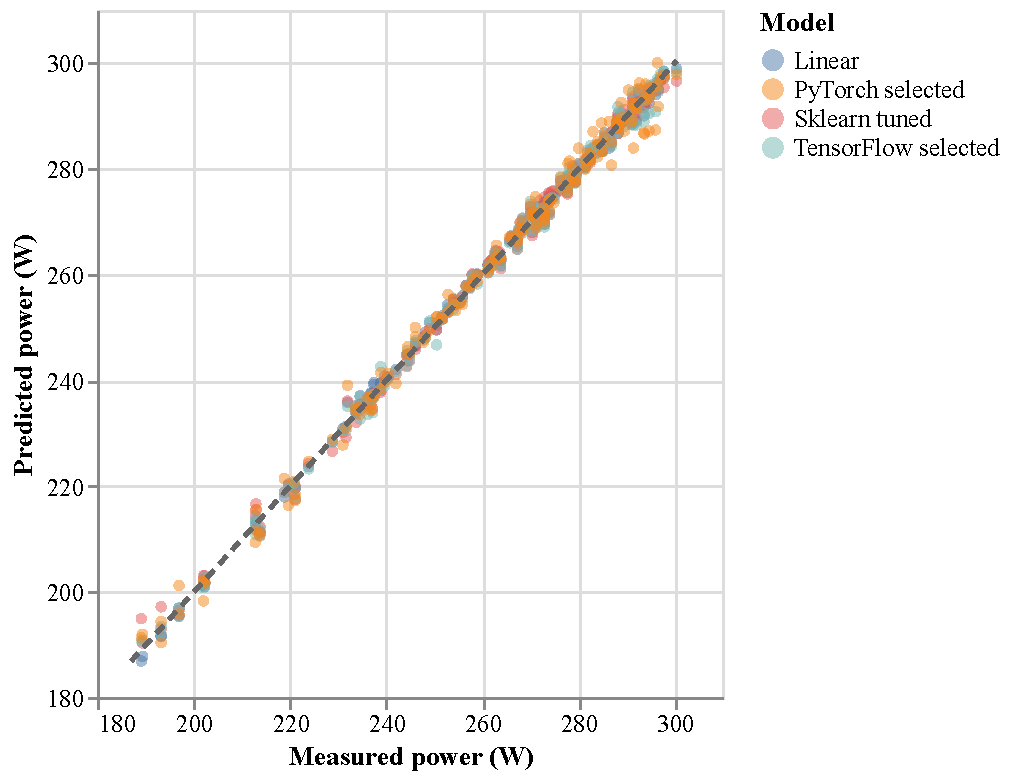
\includegraphics[width=\columnwidth]{figures/figure_A1}

\caption{Measured versus predicted power, Track A, seed 0. Each model includes all saved outer rows; dashed line is identity.}

\end{figure}

\begin{figure}[H]\centering

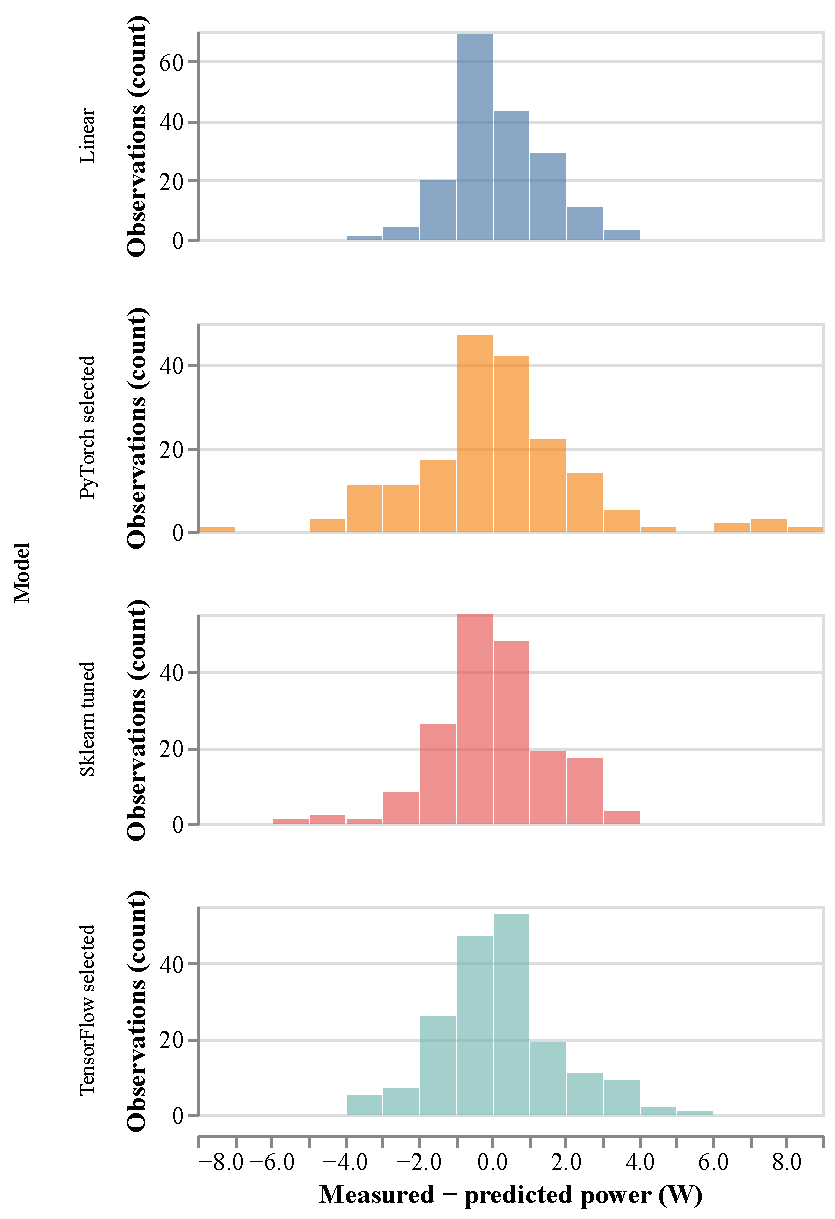
\includegraphics[width=\columnwidth]{figures/figure_A2}

\caption{Signed residual histograms, Track A, seed 0. Residual is measured minus predicted power; vertical scales vary by model.}

\end{figure}

\begin{figure}[H]\centering

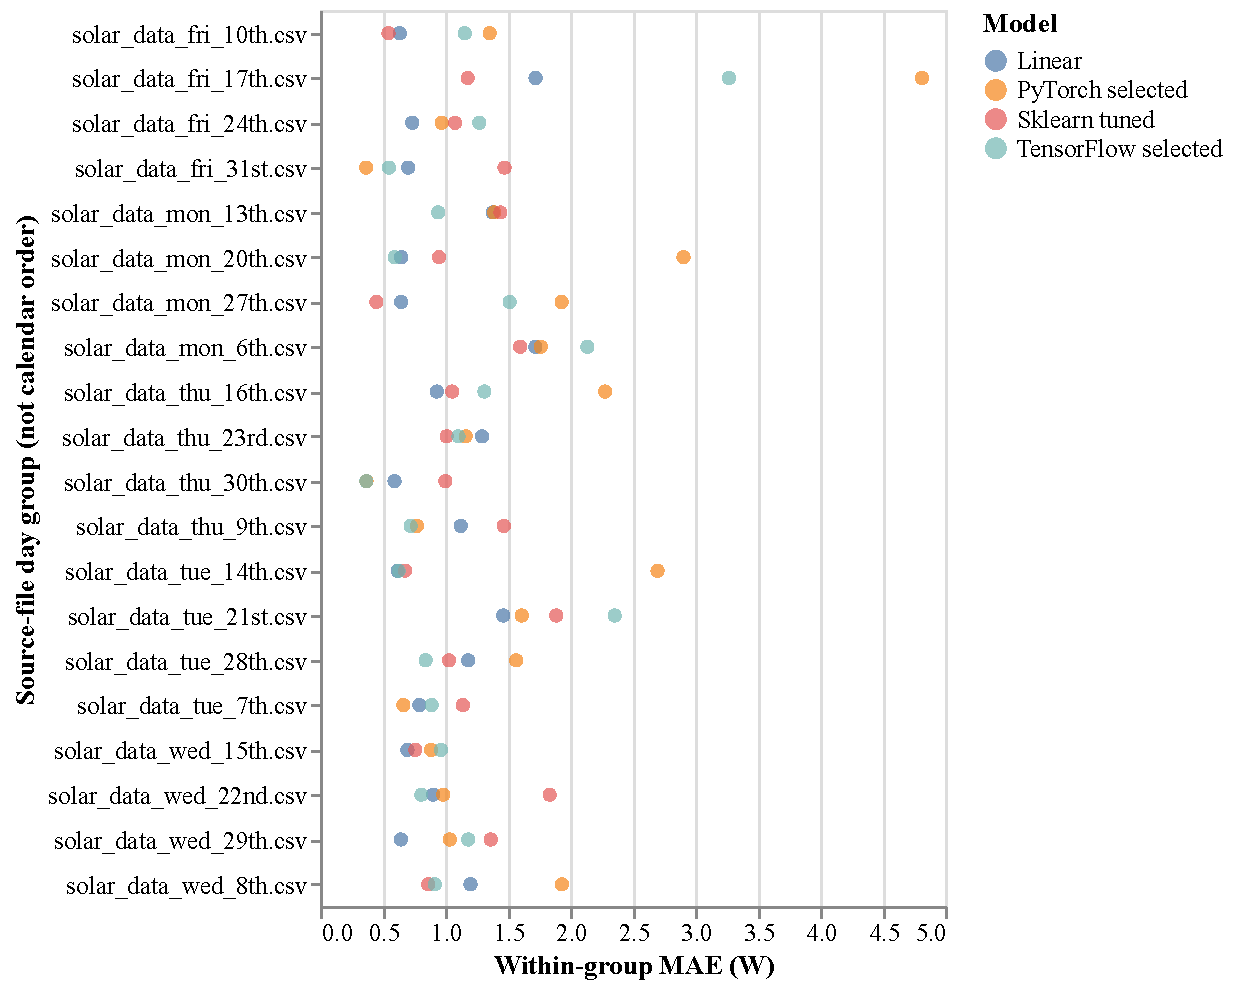
\includegraphics[width=\columnwidth]{figures/figure_A3}

\caption{Within-source-group MAE, Track A, seed 0. Filename order is categorical, not chronological; each point averages nine stored readings.}

\end{figure}

\begin{figure}[H]\centering

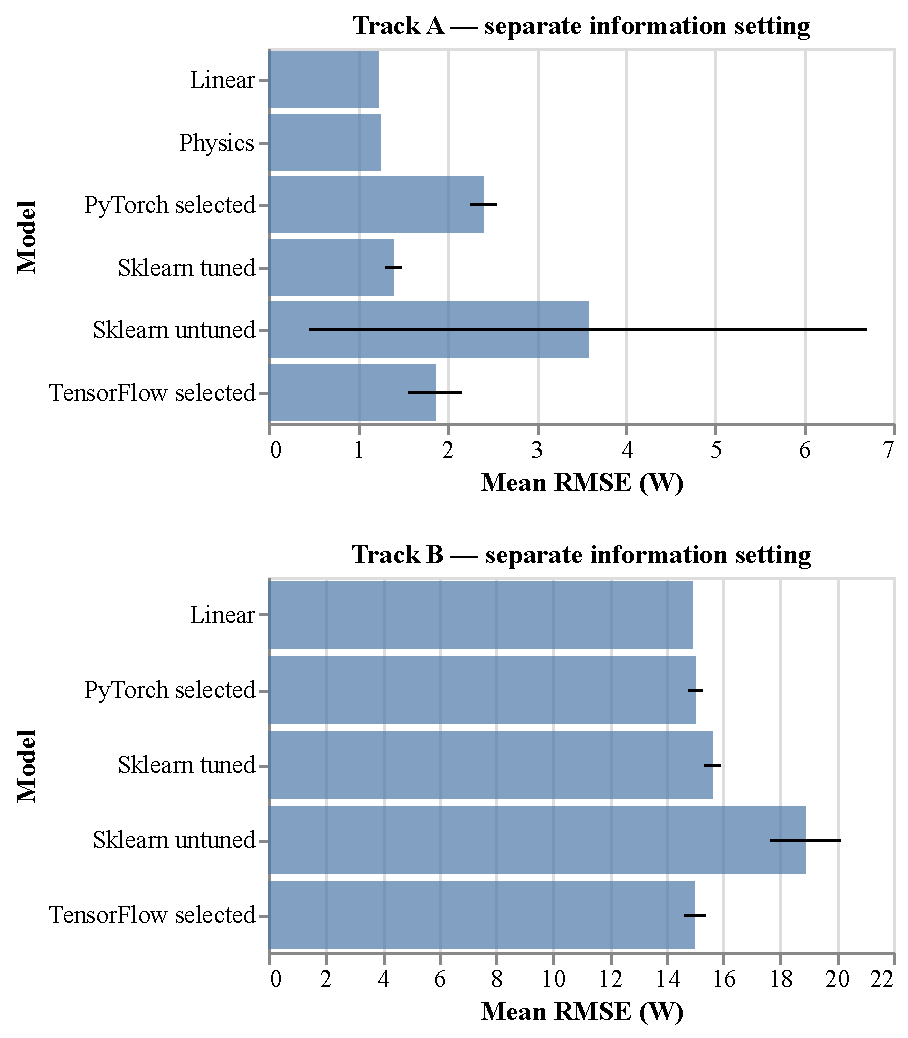
\includegraphics[width=\columnwidth]{figures/figure_A4}

\caption{Matched S2 mean RMSE with one population seed standard deviation. Track panels have independent scales; bars start at zero.}

\end{figure}

\begin{figure}[H]\centering

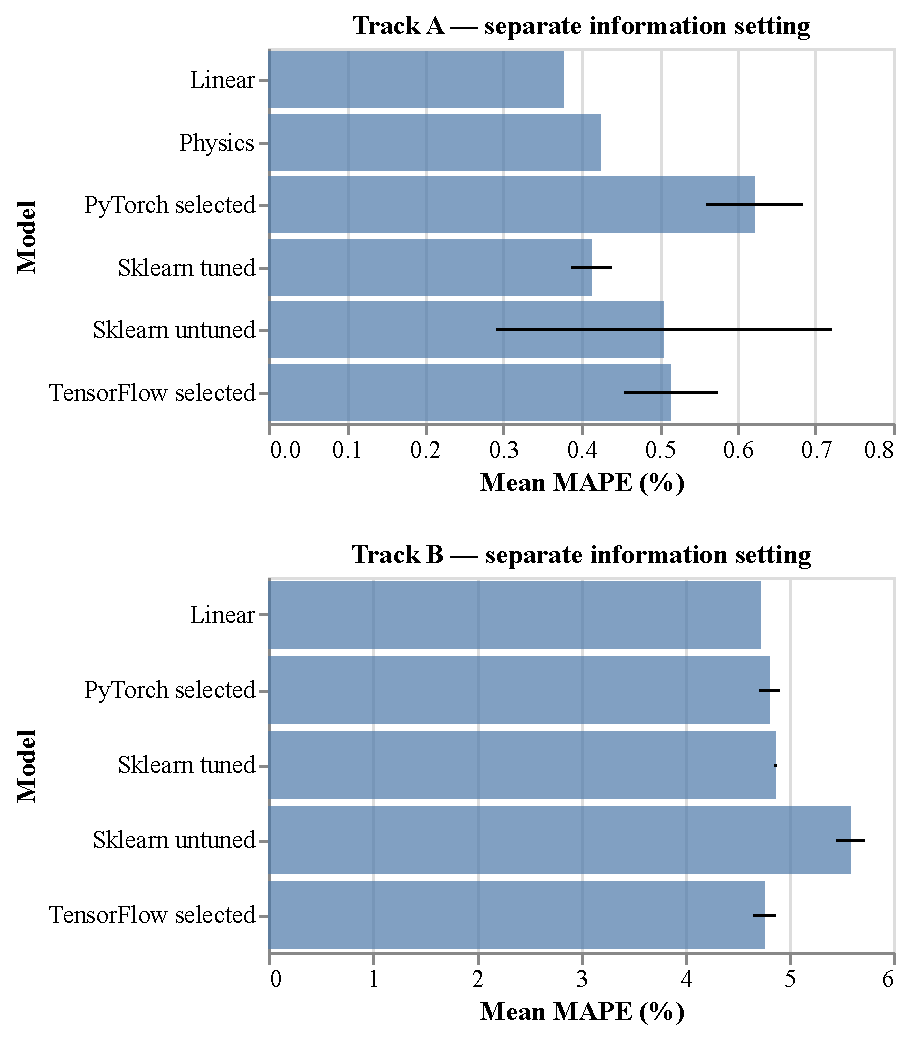
\includegraphics[width=\columnwidth]{figures/figure_A5}

\caption{Matched S2 mean MAPE with one population seed standard deviation. Track panels have independent scales; bars start at zero.}

\end{figure}

\begin{thebibliography}{6}

\bibitem{ref1} O. Ibrahim, ``Forecasting Solar Power Generation using Artificial Neural Networks,'' SSRN preprint, manuscript dated May 25, 2023; posted Apr. 18, 2024. doi: 10.2139/ssrn.4771898. \url{https://doi.org/10.2139/ssrn.4771898}

\bibitem{ref2} J. Antonanzas, N. Osorio, R. Escobar, R. Urraca, F. J. Martinez-de-Pison, and F. Antonanzas-Torres, ``Review of photovoltaic power forecasting,'' Solar Energy, vol. 136, pp. 78--111, 2016. doi: 10.1016/j.solener.2016.06.069. \url{https://doi.org/10.1016/j.solener.2016.06.069}

\bibitem{ref3} K. Hornik, M. Stinchcombe, and H. White, ``Multilayer feedforward networks are universal approximators,'' Neural Networks, vol. 2, no. 5, pp. 359--366, 1989. doi: 10.1016/0893-6080(89)90020-8. \url{https://doi.org/10.1016/0893-6080(89)90020-8}

\bibitem{ref4} S. Kaufman, S. Rosset, C. Perlich, and O. Stitelman, ``Leakage in data mining: Formulation, detection, and avoidance,'' ACM Transactions on Knowledge Discovery from Data, vol. 6, no. 4, Art. 15, 2012. doi: 10.1145/2382577.2382579. \url{https://doi.org/10.1145/2382577.2382579}

\bibitem{ref5} D. R. Roberts et al., ``Cross-validation strategies for data with temporal, spatial, hierarchical, or phylogenetic structure,'' Ecography, vol. 40, no. 8, pp. 913--929, 2017. doi: 10.1111/ecog.02881. \url{https://doi.org/10.1111/ecog.02881}

\bibitem{ref6} G. C. Cawley and N. L. C. Talbot, ``On over-fitting in model selection and subsequent selection bias in performance evaluation,'' Journal of Machine Learning Research, vol. 11, pp. 2079--2107, 2010. \url{https://www.jmlr.org/papers/v11/cawley10a.html}

\end{thebibliography}

\end{document}
